\documentclass[border=4pt]{standalone}
\usepackage{fontspec}
\usepackage{amsmath}
\usepackage{unicode-math}
\setmainfont{Latin Modern Roman}
\setmathfont{Latin Modern Math}
\usepackage{pgfplots}
\usepackage{pgfplotstable}
\pgfplotsset{compat=1.18}
\usepackage{tkz-euclide}
\usetikzlibrary{arrows.meta,calc,angles,quotes,patterns,3d,backgrounds}
\definecolor{ink}{HTML}{123428}
\definecolor{asy}{HTML}{475569}
\definecolor{mint}{HTML}{86e0bd}
\tikzset{asym/.style={asy, line width=0.9pt, dash pattern=on 5pt off 3.5pt},
         guide/.style={gray!70, line width=0.6pt, densely dotted},
         dot/.style={circle, inner sep=0pt, minimum size=5pt, draw=white, line width=0.5pt},
         odot/.style={circle, inner sep=0pt, minimum size=5.5pt, fill=white, line width=1pt},
         lab/.style={font=\footnotesize, inner sep=1.5pt, text=ink}}
\begin{document}
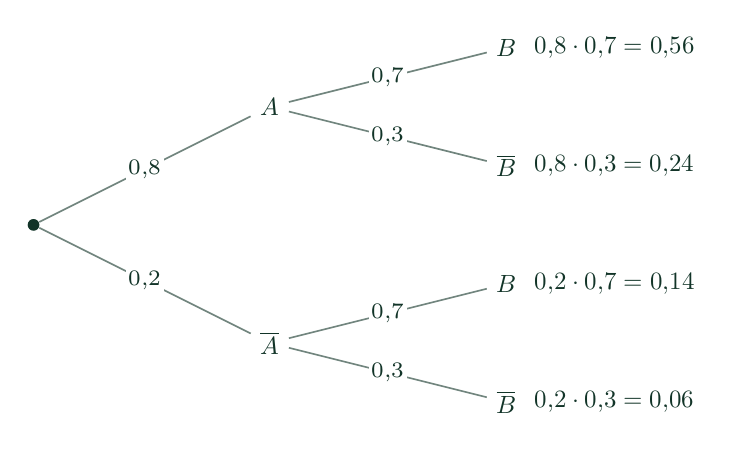
\begin{tikzpicture}[grow=right, level distance=3cm, level 1/.style={sibling distance=3cm}, level 2/.style={sibling distance=1.5cm},
  every node/.style={font=\small, text=ink}, edge from parent/.style={draw=ink!60, line width=0.6pt}, el/.style={font=\footnotesize, fill=white, inner sep=1pt}]
\node[circle, fill=ink, inner sep=1.5pt] {}
  child {node {$\overline A$} child {node[label={[text=ink]right:$0{,}2\cdot0{,}3=0{,}06$}] {$\overline B$} edge from parent node[el] {$0{,}3$}} child {node[label={[text=ink]right:$0{,}2\cdot0{,}7=0{,}14$}] {$B$} edge from parent node[el] {$0{,}7$}} edge from parent node[el] {$0{,}2$}}
  child {node {$A$} child {node[label={[text=ink]right:$0{,}8\cdot0{,}3=0{,}24$}] {$\overline B$} edge from parent node[el] {$0{,}3$}} child {node[label={[text=ink]right:$0{,}8\cdot0{,}7=0{,}56$}] {$B$} edge from parent node[el] {$0{,}7$}} edge from parent node[el] {$0{,}8$}};
\end{tikzpicture}
\end{document}
